\documentclass{article}

\usepackage{calculator}
\usepackage{calculus}

\usepackage{fancyhdr}
\usepackage{extramarks}
\usepackage{amsmath}
\usepackage{amsthm}
\usepackage{amsfonts}
\usepackage{tikz}
\usepackage[plain]{algorithm}
\usepackage{algpseudocode}
\usepackage{tikz,pgfplots,multicol}
\usepackage[font=small,labelformat=empty]{caption}
\usetikzlibrary{automata,positioning,arrows,patterns}

%
% Basic Document Settings
%

\topmargin=-0.45in
\evensidemargin=0in
\oddsidemargin=0in
\textwidth=6.5in
\textheight=9.0in
\headsep=0.25in

\linespread{1.1}

\pagestyle{fancy}
\lhead{\hmwkAuthorName}
\chead{\hmwkClass\ (\hmwkClassInstructor\ \hmwkClassTime)}
\rhead{\hmwkTitle}
\lfoot{\lastxmark}
\cfoot{\thepage}

\renewcommand\headrulewidth{0.4pt}
\renewcommand\footrulewidth{0.4pt}

\setlength\parindent{0pt}

\setcounter{secnumdepth}{0}
\newcounter{partCounter}
\newcounter{homeworkProblemCounter}
\setcounter{homeworkProblemCounter}{1}
\nobreak\extramarks{Problem \arabic{homeworkProblemCounter}}{}\nobreak{}

%
% Homework Problem Environment
%
% This environment takes an optional argument. When given, it will adjust the
% problem counter. This is useful for when the problems given for your
% assignment aren't sequential. See the last 3 problems of this template for an
% example.
%
\newenvironment{homeworkProblem}[1][-1]{
    \ifnum#1>0
        \setcounter{homeworkProblemCounter}{#1}
    \fi
    \section{Problem \arabic{homeworkProblemCounter}}
    \setcounter{partCounter}{1}
    \enterProblemHeader{homeworkProblemCounter}
}{
    \exitProblemHeader{homeworkProblemCounter}
}

%
% Homework Details
%   - Title
%   - Due date
%   - Class
%   - Section/Time
%   - Instructor
%   - Author
%

\newcommand{\hmwkTitle}{HW \#6}
\newcommand{\hmwkDueDate}{February 23, 2017}
\newcommand{\hmwkClass}{MATH 1300}
\newcommand{\hmwkClassTime}{Section 005}
\newcommand{\hmwkClassInstructor}{Professor Braden Balentine}
\newcommand{\hmwkAuthorName}{\textbf{John Keller}}

%
% Title Page
%

\title{
    \vspace{2in}
    \textmd{\textbf{\hmwkClass:\ \hmwkTitle}}\\
    \normalsize\vspace{0.1in}\small{Due\ on\ \hmwkDueDate\ at 10:00am}\\
    \vspace{0.1in}\large{\textit{\hmwkClassInstructor\ \hmwkClassTime}}
    \vspace{3in}
}

\author{\hmwkAuthorName}
\date{}

\renewcommand{\part}[1]{\textbf{\large Part \Alph{partCounter}}\stepcounter{partCounter}\\}

%
% Various Helper Commands
%

% Useful for algorithms
\newcommand{\alg}[1]{\textsc{\bfseries \footnotesize #1}}

% For derivatives
\newcommand{\deriv}[1]{\frac{\mathrm{d}}{\mathrm{d}x} (#1)}

% For partial derivatives
\newcommand{\pderiv}[2]{\frac{\partial}{\partial #1} (#2)}

% Integral dx
\newcommand{\dx}{\mathrm{d}x}

% Alias for the Solution section header
\newcommand{\solution}{\textbf{\large Solution}}

% Probability commands: Expectation, Variance, Covariance, Bias
\newcommand{\E}{\mathrm{E}}
\newcommand{\Var}{\mathrm{Var}}
\newcommand{\Cov}{\mathrm{Cov}}
\newcommand{\Bias}{\mathrm{Bias}}


\usepackage{xcolor}
    \colorlet{Curve}{red!75!black}
    \colorlet{Tangent}{blue!75!black}
\usepackage{pgfplots}
    \pgfplotsset{compat=1.10}
    \usetikzlibrary{
        calc,
        intersections,
        math,
    }
    \makeatletter
        \def\parsenode[#1]#2\pgf@nil{%
            \tikzset{label node/.style={#1}}
            \def\nodetext{#2}
        }
        \tikzset{
            % define style for the points
            Point/.style={
                shape=circle,
                inner sep=0pt,
                minimum size=3pt,
            },
            add node at x/.style 2 args={
                name path global=plot line,
                /pgfplots/execute at end plot visualization/.append={
                        \begingroup
                        \@ifnextchar[{\parsenode}{\parsenode[]}#2\pgf@nil
                    \path [name path global = position line #1-1]
                        ({axis cs:#1,0}|-{rel axis cs:0,0}) --
                        ({axis cs:#1,0}|-{rel axis cs:0,1});
                    \path [xshift=1pt, name path global = position line #1-2]
                        ({axis cs:#1,0}|-{rel axis cs:0,0}) --
                        ({axis cs:#1,0}|-{rel axis cs:0,1});
                    \path [
                        name intersections={
                            of={plot line and position line #1-1},
                            name=left intersection
                        },
                        name intersections={
                            of={plot line and position line #1-2},
                            name=right intersection
                        },
                        label node/.append style={pos=1}
                    ] (left intersection-1) -- (right intersection-1)
                        node [label node]{\nodetext};
                    % ---------------------------------------------------------
                    % draw the tangent line from a bit right of the point on
                    % the curve to the intersection with the ordinate
                    % and draw the corresponding points
                    \draw [dashed] let
                        \p1=($ (left intersection-1) - (right intersection-1) $),
                        \p2=($ (left intersection-1)!sign(#1)*10mm!(right intersection-1) $),
                        %\p2=($ (left intersection+1) - (right intersection+1) $),
                        \p3=($ ({axis cs:0,0}) - (\p2) $),
                        \n1={\x3/\x1}	% slope of tangent line
                    in
                        (\p2) -- +($ {\n1}*(\x1,\y1) $)
	                        
%                        		node[right,node font=\scriptsize,gray] {$y=$\y1/\x1*sign(#1) $x+$}
%                            node [Point,fill=Tangent] (origin intersection) {}
                            node [Point,fill=Curve] at (left intersection-1) {}
                    ;
                    % ----------
                    % draw the horizontal line at the curve intersection point
                    % plus the label above/below the line
%                    \tikzmath{
%                        coordinate \c1;
%                        \c1=(left intersection-1) - (right intersection-1);
%                        \slope=\cy1/\cx1*sign(#1);
%                        \plusoffset = (#1+1);
%                    }
%                    \pgfmathsetmacro{\AboveBelow}{ \slope>0 ? "above" : "below" }
%                    \draw [dashed]
%                        ([xshift=sign(#1)*2.5mm] left intersection-1) --
%                        (left intersection-1) --
%                            node [\AboveBelow,node font=\scriptsize] {$y=\slope x+\plusoffset$}
%                        (left intersection-1 -| origin intersection) --
%                        +($ sign(#1)*(-2.5mm,0) $)
%                            coordinate [pos=0.5] (a)
%                    ;
%                    % draw the horizontal line at the ordinate intersection point
%                    \draw [dotted] (origin intersection)
%                        +($ sign(#1)*(-2.5mm,0) $) --
%                        (origin intersection);
%                    % draw vertical line left/right of the ordinate
%                    \pgfmathsetmacro{\LeftRight}{ #1<0 ? "right" : "left" }
%                    \draw [stealth-stealth] (origin intersection)
%                        +($ sign(#1)*(-1.25mm,0) $) -- (a)
%                            node [midway,\LeftRight,node font=\scriptsize] {$p$}
%                    ;
%                    % ---------------------------------------------------------
                        \endgroup
                },
            },
        }
    \makeatother
\makeatletter
\def\mathcolor#1#{\@mathcolor{#1}}
\def\@mathcolor#1#2#3{%
  \protect\leavevmode
  \begingroup
    \color#1{#2}#3%
  \endgroup
}
\makeatother


\begin{document}

\maketitle

\pagebreak

\section{Additional Problems for Homework 6}
\begin{center}
	
	\begin{minipage}[t]{0.49\linewidth}
	\vspace{0pt}
	A graph of $f(x)$ is shown below.\\ It is piecewise linear.\newline\newline
		\pgfplotsset{width=6cm,height=5cm,xmin=-2, ymax=5, axis equal,xtick={1,2,3,4},yticklabels={ , , ,4},ytick={1,2,3,4}}
%		\pgfplotsset{xmin=-10,xmax=10,ymin=-4,ymax=6,soldot/.style={color=blue,only marks,mark=*}
			\begin{tikzpicture}
			\begin{axis}[axis lines=middle,minor y tick num=0,minor x tick num=0,tick style={black},grid style={solid, gray!20}]
				\addplot[domain=0:2] {x+2};
				\addplot[domain=2:5][->] {-2*x+8};
				\addplot+[only marks,mark=*,mark options={fill=black,scale=0.7},text mark as node=false,black] coordinates {(0,2)(2,4)(4,0)};
			\end{axis}
		\end{tikzpicture}
	\end{minipage}
	\begin{minipage}[t]{0.49\linewidth}
	\vspace{0pt}
		The table below gives values of $g(x)$ and $g'(x)$.\newline\newline
				\begin{tabular}{c|c|c|c|c|c}
		        $x$     & 0 & 1 & 2 & 3  & 4  \\ \hline
		        $g(x)$  & 2 & 5 & 9 & 11 & 8  \\ \hline
		        $g'(x)$ & 3 & 4 & 3 & -3 & -4 
				\end{tabular}
	\end{minipage}
\end{center}

\begin{enumerate}
	\item Given $h(x)=f(x)g(x)$, find $h'(1)$.
	$$\begin{align}
		h'(1)&= f'(1)g(1) + f(1)g'(1) \\
		&= 1\cdot 5 + 3 \cdot 4 \\
		&= 5 + 12\\
		&= 17
	\end{align}$$
	\item Given $k(x)=\frac{f(x)}{g(x)}$, find $k'(3)$.
	$$\begin{align}
		k'(3) &= \frac{f'(3)g(3) - f(3)g'(3)}{[g(3)]^2} \\
		&= \frac{-2 \cdot 11 - 2 \cdot -3}{11^2} \\
		&= \frac{-22 + 6}{11^2} \\
		&= \FRACTIONSIMPLIFY{-16}{121}{\num}{\den} \frac{\num}{\den}\\
	\end{align}$$
	\item Given $\ell(x)=\frac{g(x)}{\sqrt{x}}$, find $\ell'(4)$.
	$$\begin{align}
		\ell'(4) &= \frac{g'(4)\sqrt{4} - g(4)\cdot 0}{4} \\
		&= \frac{-4 \cdot 2 - 8 \cdot 0}{4} \\
		&= \frac{-8-0}{4} \\
		&= -2
		% tempA = 
	\end{align}$$
\end{enumerate}
\pagebreak
\section{Section 3.2}

\begin{enumerate}
\setcounter{enumi}{47}
	\item If $f$ is a differentiable function, find an expression for the derivative:
		\begin{enumerate}
			\setcounter{enumii}{3}
			\item $y=\frac{1+xf(x)}{\sqrt{x}}$.
			$$\begin{align}
				y &= \frac{\big(0+f(x)+xf'(x)\big)\sqrt{x}-\big(\frac{1}{2}x^{-\frac{1}{2}}(1+xf(x))\big)}{(\sqrt{x})^2} \\
				 &= \frac{(f(x)+xf'(x))\sqrt{x}-\big(\frac{1}{2}x^{-\frac{1}{2}}+\frac{1}{2}x^{\frac{1}{2}}f(x)\big)}{x} \\
				 &= \frac{x^{\frac{1}{2}}f(x)+x^{\frac{1}{2}}f'(x)-\frac{1}{2}x^{-\frac{1}{2}}-\frac{1}{2}x^{\frac{1}{2}}f(x)}{x} \\
				 &= \frac{\frac{1}{2}x^{\frac{1}{2}}f(x)+x^{\frac{1}{2}}f'(x)-\frac{1}{2}x^{-\frac{1}{2}}}{x}\\
				 &= \frac{2xf'(x)+xf(x)-1}{2x^{\frac{2}{3}}}
			\end{align}$$
		\end{enumerate}
\setcounter{enumi}{49}
	\item A manufacturer produces bolts of a fabric with a fixed width. The quantity $q$ of this fabric (measured in years) that is sold is a unction of the selling price $p$ (in dollars per yard), so we can write $q=f(p)$. Then the total revenue earned with selling price $p$ is $R(p)=pf(p)$.
		\begin{enumerate}
			\item What does it mean to say that $f(20)=10,000$ and $f'(20)=-350$?
				\begin{itemize}
					\item When the selling price is \$20, then the quantity is 10,000 yards.
					\item At the price of \$20, the slope is -350 per dollar, meaning that for every dollar cheaper the selling price, the quantity goes down by 350 (at the exact price of \$20).
				\end{itemize}
			\item Assuming the values in part (a), find $R'(20)$ and interpret your answer.
				$$\begin{align}
					R'(p) &= p\cdot f'(p) + p' \cdot f(p)\\
						&= p\cdot f'(p) + f(p)\\
						R'(20) &= 20 \cdot f(20) + f'(20)\\
						&= 20(-350)+10,000 \\
						&= 9,300 \text{ yards}
				\end{align}$$
				Because $R'$ is the slope at only one specific point, not much can be interpreted from the value, but the positive slope can be somewhat associated with a higher revenue.
		\end{enumerate}
	\item On what interval is the function $f(x)=x^3e^x$ increasing? $\boldsymbol{(-3,\infty)}$
	\def\crulefill{\leaders\hrule
  height \dimexpr\fontdimen22\textfont2+0.2pt\relax
  depth -\dimexpr\fontdimen22\textfont2-0.2pt\relax
  \hfill
}
\def\hollow{$\kern-.8pt\circ\kern-.8pt$}
\def\filled{$\kern-.8pt\bullet\kern-.8pt$}

$$
\vbox{\offinterlineskip\tabskip=0pt
  \halign{%
    \strut$#$\hfil&
    \hfil\qquad$#$\qquad\hfil&
    \hfil\vrule#\hfil&
    \hfil\qquad$#$\qquad\hfil&
    \hfil\vrule#\hfil&
    \hfil\qquad$#$\qquad\hfil&
    \hfil\vrule#\hfil&
    \hfil\qquad$#$\qquad\hfil\cr
  & - && + && + && + \cr
  \multispan{2}\crulefill
  &\omit\hfil\filled\hfil
  &\omit\crulefill
  &\omit\hfil\filled\hfil
  &\omit\crulefill
  &\omit\hfil\filled\hfil
  &\omit\crulefill\cr
  & &\omit\hidewidth$-3$\hidewidth& &\omit\hidewidth$0$\hidewidth& &\omit\hidewidth$1$\hidewidth& \cr
}}
$$
	\item On what interval is the function $f(x)=x^2e^x$ concave downward? $\boldsymbol{(-1.5,0)}$
\setcounter{enumi}{57}
	\item 
		\begin{enumerate}
			\item If $F(x)=f(x)g(x)$, where $f$ and $g$ have derivatives of all orders, show that $F''=f''g+2f'g'+fg''$.
				$$\begin{align}
					F' &= f'\cdot g +f \cdot g' \\
					F'' &= \big(f''\cdot g'\cdot f\cdot g'\big)+\big(f'\cdot g\cdot f'\cdot g''\big)\\
					    &= f''\cdot g + 2f'\cdot g' + f\cdot g''
				\end{align}$$
			\item Find similar formulas for $F'''$ and $F^{(4)}$.
				$$\begin{align}
					F''' &=  f^{3} g + 3 f'' g' + 3 f' g'' + f g^3 \\
					F^{(4)} & = f^4 g(x) + 4 f^3 g' + 6 f'' g'' + 4 g^3 f' + f g^4
				\end{align}$$
			\item Guess a formula for $F^{(n)}$.
			$$\begin{align}
				F^{n} &= f^n\cdot g + nf^{n-1}\cdot g' + n^{\frac{1}{2}}f^{n-2}g^{n-2}+ng^{n-1}f'+fg^n
			\end{align}$$
		\end{enumerate}
\end{enumerate}

\section{Section 3.3}

\begin{enumerate}
\setcounter{enumi}{15}
	\item Prove that $\frac{d}{dx}(\text{sec}x)=\sec x \tan x$.
	$$\begin{align}
		\sec x &= \frac{1}{\cos x}\\
		\frac{d}{dx} (\sec x) &= \frac{0\cdot \cos x - (-\sin x)}{\cos^2 x}\\
		&= \frac{\sin x}{\cos x \cdot \cos x} \\
		&= \boxed{\sec x \tan x}
	\end{align}$$
\setcounter{enumi}{36}
	\item 
	\begin{center}
		\begin{minipage}[t]{0.74\linewidth}
			\vspace{-0.2cm}A ladder 10 ft long rests against a vertical wall. Let $\theta$ be the angle between the top of the ladder and the wall and let $x$ be the distance from the bottom of the ladder to the wall. If the bottom of the ladder slides away from the wall, how fast does $x$ change with respect to $\theta$ when $\theta=\frac{\pi}{3}$?
		\end{minipage}
		\begin{minipage}[t]{0.25\linewidth}
			\vspace{-0.2cm} \begin{flushright}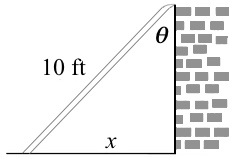
\includegraphics[height=2cm]{images/33pr37.jpg}\end{flushright}
		\end{minipage}
	\end{center}
	
	$$\begin{align}
		10^2 &= x^2 + \cos\theta \\
		x &= (100-\cos \theta)^{\frac{1}{2}} \\
		\frac{dx}{d\theta} &= \frac{1}{2}(100-\cos\theta)\sin\theta \\
		\frac{dx}{d\theta} &= \frac{1}{2}\Big(100-\frac{1}{2}\Big)\frac{\sqrt{3}}{2} \\
		\frac{dx}{d\theta} &= \frac{\sqrt{3}}{4}(99.5) \\
		\frac{dx}{d\theta} &= \boxed{\frac{\sqrt{3}\cdot 99.5}{4}}
	\end{align}$$
	
	
\end{enumerate}
Find the given derivative by finding the first few derivatives and observing the pattern that occurs.
\begin{center}
\begin{minipage}[t]{0.49\linewidth}
	\begin{enumerate}
\setcounter{enumi}{38}
	\item $\frac{d^{99}}{dx^{99}}(\sin x)$
		$$\begin{align}
			\frac{d}{dx} &= \boldsymbol{\cos x}\\
			\frac{d^2}{dx^2} &= -\sin x\\
			\frac{d^3}{dx^3} &= -\cos x\\
			\frac{d^4}{dx^4} &= \sin x\\
			\frac{d^5}{dx^5} &= \boldsymbol{\cos x}\\
			\frac{d^9}{dx^9} &= \frac{d}{dx}\\
			\frac{d^{97}}{dx^{97}} &= \frac{d}{dx}\\
			\frac{d^{99}}{dx^{99}} &= \frac{d^3}{dx^3} = \boxed{-\cos x}
		\end{align}$$
\end{enumerate}
\end{minipage}
\begin{minipage}[t]{0.49\linewidth}
\begin{enumerate}
\setcounter{enumi}{39}
	\item $\frac{d^{35}}{dx^{35}}(x\sin x)$
	$$\begin{align}
		\frac{d}{dx}&= \boldsymbol{1}\sin x + x \cos x\\
		\frac{d^2}{dx^2} &= \boldsymbol{2}\cos x - \sin x\\
		\frac{d^3}{dx^3} &= \boldsymbol{-3}\sin x - x \cos x \\
		\frac{d^4}{dx^4} &= x\sin x \boldsymbol{- 4} \cos x\\
		\frac{d^5}{dx^5} &= \boldsymbol{5}\sin x + x \cos x\\
		\frac{d^6}{dx^6} &= \boldsymbol{6}\cos x - x \sin x\\
		\frac{d^{35}}{dx^{35}} &= \boxed{-x \cos x \boldsymbol{-35}\sin x}
	\end{align}$$
\end{enumerate}
\end{minipage}
\end{center}


\end{document}